\documentclass[12pt]{article}

\usepackage{sbc-template}

\usepackage{graphicx,url}

\usepackage[brazil]{babel}   
%\usepackage[latin1]{inputenc}  

\usepackage{tikz}
\usepackage{xcolor,xspace}
\usepackage{thmtools}
\usepackage{amsmath,amssymb}
\usepackage{mathpartir}
\usepackage{lettrine}
\usepackage[modulo]{lineno}
\usepackage{lipsum}

\newcommand{\auxFun}[1]{\mbox{\textbf{#1}}}
\newcommand\loc[1]{\mbox{\textsf{loc}$_{#1}$}}
\newcommand\gr{\xspace\mbox{GR}\xspace}
\newcommand\lr{\xspace\mbox{LR}\xspace}
\newcommand{\cupdot}{\mathbin{\mathaccent\cdot\cup}}
\newcommand\supp{\xspace\mbox{supp}\xspace}
\newcommand{\lb}[1]{\mbox{$#1$}_{\downarrow}}
\newcommand{\ub}[1]{\mbox{$#1$}_{\uparrow}}     

\sloppy

\title{Symbolic Range Analysis of Pointers\\ Dissertation Summary}

\author{Vitor Mendes paisante\\Advisor: Fernando Magno Quintão Pereira\\Co-advisor: Leonardo Barbosa e Oliveira}


\address{Federal University od Minas Gerais Computer Science Department
  \email{\{paisante\}@dcc.ufmg.br}
}

\begin{document} 

\maketitle

\begin{abstract}
Alias analysis is one of the most fundamental techniques that
compilers use to optimize languages with pointers.
However, in spite of all the attention that this topic has received, the current
state-of-the-art approaches inside compilers still face challenges regarding
precision and speed.
In particular, pointer arithmetic, a key feature in C and C++, is yet to be
handled satisfactorily.
This work presented a new alias analysis algorithm to solve this problem.
The key insight of our approach was to combine alias analysis with symbolic
range analysis.
This combination allowed us to disambiguate fields within arrays and structs,
effectively achieving more precision than traditional algorithms.
To validate our technique, we implemented it on top of the LLVM compiler.
Tests on a vast suite of benchmarks showed that we could disambiguate several
kinds of C idioms that current state-of-the-art analyses could not deal with.
In particular, we could disambiguate 1.35x more queries than the alias analysis
that was currently available in LLVM.
Furthermore, our analysis was very fast: we were able go over one million assembly
instructions in 10 seconds..
\end{abstract}
     

\section {Introduction}
% the importance of Alias Analysis
Pointer analysis is one of the most fundamental compiler technologies.
This analysis lets the compiler distinguish one memory location from others;
hence, it provides the necessary information to transform code that manipulates
memory.
Given this importance, it comes as no surprise that pointer analysis has been
one of the most researched topics within the field of compiler
construction\cite{Hind01}.
This research has contributed to make the present algorithms more
precise~\cite{Hardekopf07a,Zhang14}, and faster~\cite{Hardekopf11,Shang12}.
Nevertheless, one particular feature of imperative programming languages remained
to be handled satisfactorily by the current state-of-the-art approaches:
the disambiguation of pointer intervals.

% The problem imposed by pointer arithmetics and The need for better alias analyses.
Mainstream compilers still struggle to distinguish intervals within the
same array.
In other words, state-of-the-art pointer analyses often fail to disambiguate
regions addressed from a common base pointer via different
offsets, as explained by Yong and Horwitz~\cite{Yong04}. Figure 
\ref{fig:intro_ex} shows an example that state-of-the-art pointer analyses 
tend not to deal with satisfactorily. In the example, both stores on the $r$ 
array posses different offsets and they do not alias. To figure out that such 
offsets are disjoint it is necessary to verify their ranges and add a new layer
of analysis to the current pointer analyses available.

\begin{figure}[th]
  \centering
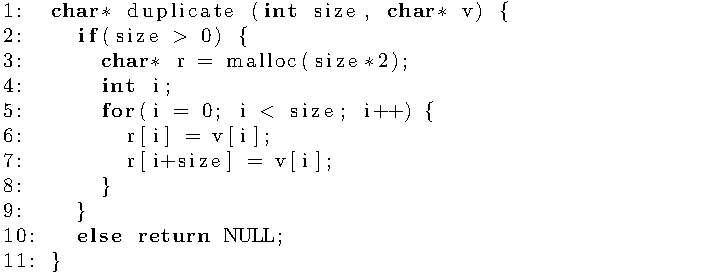
\includegraphics[width=320px]{img/introex}
  \caption{Example that state-of-the-art pointer analyses handle 
  unsatisfactorily.}
  \label{fig:intro_ex}
\end{figure}

Field-sensitive pointer analysis, provide a partial solution to this problem.
These analyses can distinguish different fields within a record, such
as a struct in C~\cite{Pearce04}, or a class in Java~\cite{Yan11}.
However, they rely on syntax that is usually absent in the low level program
representations adopted by compilers.
Shape analyses~\cite{Jones82,Sagiv98} can disambiguate subparts of
data-structures such as arrays, yet their scalability remains an issue to be
solved.
Consequently, many compiler optimizations, such as
loop transformations, tiling, fission, skewing and
interchanging~\cite[Ch.09]{Wolfe96}, are very limited in practice.
Therefore, we claim that, to reach their full potential, compilers need to
be provided with more effective alias analyses.

% Combining alias and range analyses.
This dissertation described such an analysis.
We introduced an abstract domain that associates pointers with symbolic ranges.
In other words, for each pointer $p$ we conservatively estimate the range of
memory slots that can be addressed as an offset of $p$.
We let $>(p)$ be the global abstract address set associated with pointer $p$, 
such that if
$\loc{i} + [l, u] \in >(p)$, then $p$ may dereference any address
from $@(\loc{i}) + l$ to $@(\loc{i}) + u$,
where $\loc{i}$ is a program site that
contains a memory allocation call, and $@(\loc{i})$ is the actual return
address of the {\em malloc} at runtime.
We let $\{ l, u \}$ be two {\em symbols} defined within the program code.
Like the vast majority of pointer analyses available in the compiler
literature, from Andersen's work~\cite{Andersen94} to the more recent 
technique of Zhang {\em et al.}~\cite{Zhang14}, our method is correct if the
underlying program is also correct.
In other words, our results are sound with respect to the semantics of the
program if this program has no undefined behavior, such as out-of-bounds
accesses.

\textbf{The key insight of our research} was the combination of pointer analysis
with range analysis on the symbolic interval lattice.
In a symbolic range analysis, ranges are defined as expressions of the program's
symbols, a symbol being either a constant or the name of a variable.
There exist many approaches to symbolic range analyses in the
literature~\cite{Blume94,Nazare14,Rugina05}.
The algorithms that we presented in this work do not depend on any particular
implementation.
Nevertheless, the more precise the range analysis that we use, the more
precise the analysis facts that we produce.
In this work we adopted the symbolic range analysis proposed in 1994 by
William Blume and Rudolf Eigenmann~\cite{Blume94}.

\section{Analysis Overview}
\label{sec:ovf}

We have two different ways to answer the
following question: ``do pointers $\mathit{tmp}_i$ and $\mathit{tmp}_j$
alias?"
These tests are called {\em global} and {\em local}.
In this section, we will use two different examples to illustrate situations
in which each query is more effective.
These distinct strategies are complementary: one is not a superset of the other.

\noindent
\textbf{Global pointer disambiguation. }
Figure~\ref{fig:exmotiv} illustrates our first approach to disambiguate
pointers.
The figure shows a pattern typically found in distributed systems
implemented in C.
Messages are represented as arrays of bytes.
In this particular example, messages have two parts: an identifier, which is stored in the beginning of the array, and a payload, which is stored right
after.
The loops in lines 5-8 and 9-12 fill up each of these parts with data.
If a compiler can prove that the stores at lines 6 and 10 are always
independent, then it can perform optimizations that would not be
possible otherwise.
For instance, it can parallelize the loops, or switch them, or merge them into a
single body.

\begin{figure}[t]
  \centering
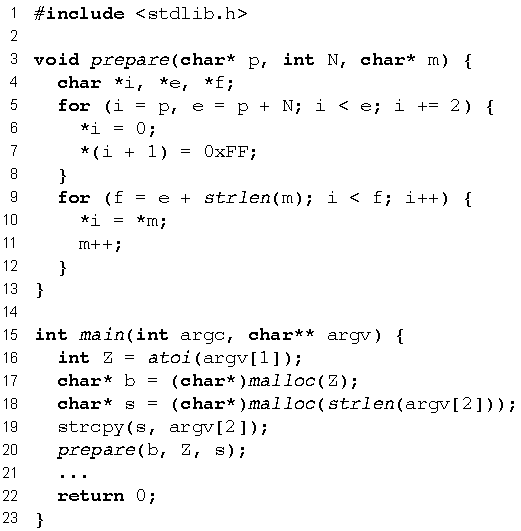
\includegraphics{img/ex0_src.pdf}
  \caption{Example of program that builds up messages as sequences of
  serialized bytes. We are interested in disambiguating the locations accessed
  at lines 6 and 10.}
  \label{fig:exmotiv}
\end{figure}

No alias analysis currently available in either gcc or LLVM is able to
disambiguate the stores at lines 6 and 10.
These analyses are limited because they do not contain {\em range information}.
The range interval $[l, u]$ associated with a variable $i$ is
an estimate of
the lowest ($l$) and highest ($u$) values that $i$ can assume
throughout the execution of the program.
In this work, we proposed an alias analysis that solves this problem.
To achieve this goal, we coupled this alias analysis with range
analysis on symbolic intervals~\cite{Blume94}.
Thus, we can say that the store at line 6 might modify any address from
$\mathtt{p} + 0$ to $\mathtt{p} + \mathtt{N} - 1$, and that the store at line 10
might write on any address from $\mathtt{p} + N$ to $\mathtt{p} + N + 
\mathtt{strlen(m) - 1}$.
For this purpose, we use an \emph{abstract address} that
encodes the actual value(s) of $p$ inside the $\mathtt{prepare}$
function.
These memory addresses are depicted in Figure \ref{fig:pointer_range}, where each
square represents a memory slot.

\begin{figure}[t!]
\begin{small}
  \centering
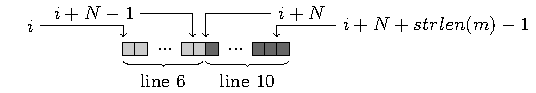
\includegraphics{img/pointer_range_Maroua}
  \caption{Array $p$ in the routine \texttt{prepare} seen in
    Fig.\ref{fig:exmotiv}. Lines 6 and 10 represent the different stores in the figure.}
  \label{fig:pointer_range}
\end{small}
\end{figure}

% How to disambiguate queries:
Whole program analysis reveals that there are two candidate locations
that any pointer in the program may refer to.
These locations have been created at lines 17 and 18 of Figure~\ref{fig:exmotiv},
and we represent them abstractly as $\loc{17}$ and  $\loc{18}$.
These names are unique across the entire program.
After running our analysis, we find out that the abstract state ($\gr$) of
\texttt{i} at line 6 is
$\gr(\mathtt{i}_{\ell{}n.6}) = \{ \loc{17} + [0, \mathtt{N} - 1]$,
and that the abstract state of \texttt{i} at line 10 is
$\gr(\mathtt{i}_{\ell{}n.10}) = \{ \loc{17} + [\mathtt{N}, \mathtt{N + strlen}(m) - 1]
\}$.
Given that these two abstract ranges do not intersect, we know that
the two stores update always different locations.
We call this check the {\em global disambiguation
  criterion}.

\begin{figure}[t!]
  \centering
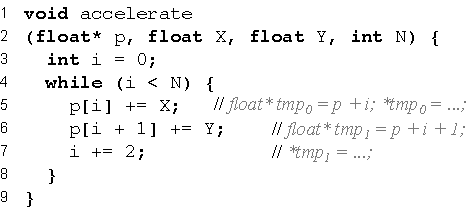
\includegraphics{img/ex4_src}
  \caption{Program that shows the need to assign common names to addresses that spring from the same base pointer.}
  \label{fig:ex4_src}
\end{figure}

\begin{figure}[t!]
  \centering
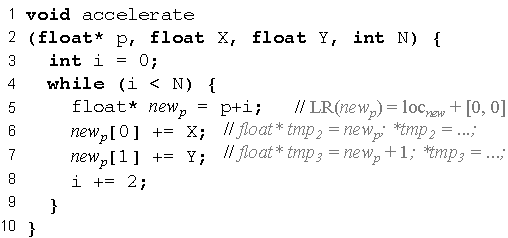
\includegraphics{img/ex4_norm}
  \caption{Program from Figure~\ref{fig:ex4_src}, after pointer is renamed
  within loop.}
  \label{fig:ex4_norm}
\end{figure}

\textbf{Local pointer disambiguation. } Figure~\ref{fig:ex4_src} shows
a program in which the simple intersection of ranges would not let us
disambiguate pointers $\mathit{tmp}_0$ and $\mathit{tmp}_1$.  After
solving global range analysis for that program, we have that
$\gr(\mathit{tmp}_0) = \{ \loc{0} + [0, N + 1] \}$ and that
$\gr(\mathit{tmp}_1) = \{ \loc{0} + [1, N + 2] \}$, where $\loc{0}$
defines the abstract address of the function parameter $p$.  The
intersection of these ranges is non-empty for $N \geq 1$.  Thus, the
global check that we have used to disambiguate locations in
Figure~\ref{fig:exmotiv} does not work in Figure~\ref{fig:ex4_src}.
Notwithstanding this fact, we know that $\mathit{tmp}_0$ and
$\mathit{tmp}_1$ will never point to a common location.  In fact,
these pointers constitute different offsets from the same base
address.
To deal with this imprecision of the global check, we will be also discussing
a {\em local disambiguation criterion}.
In this case, we rename every pointer $p$ that is alive at the beginning of
a single entry region to a fresh name $new_{p}$.
Whereas we use the global test for pointers in different regions, the
local test is applied onto pointers within the same single entry region.
After renaming, we update the table of pointer pairs, so that
$\lr(new_p) = \loc{new} + [0, 0]$, regardless of the old ranges assigned to
the original pointer $p$.
In Figure~\ref{fig:ex4_norm} we would have that
$\lr(\mathit{tmp}_2) =  \loc{new} + [0, 0]$  and
$\lr(\mathit{tmp}_3) =  \loc{new} + [1, 1]$, where $\mathit{tmp_2}$ is
the name of the address $\mathit{new}_p[0]$, and
$\mathit{tmp_3}$ is the name of the address $\mathit{new}_p[1]$.
This new binding of intervals to pointers gives us empty
intersections between similar locations in $\lr(tmp_2)$ and $\lr(tmp_3)$.
Consequently, the local check is able to distinguish addresses referenced by
$\mathit{tmp}_2$ and $\mathit{tmp}_3$.

\section {Summary of experimental results}
To validate our ideas, we implemented them in the LLVM compilation
infra-structure~\cite{Lattner04}.
We tested our pointer analysis onto three different benchmarks
used in previous work related to pointer disambiguation:
Prolangs~\cite{Ryder01}, PtrDist~\cite{Zhao05} and MallocBench~\cite{Grunwald93}.
Our analysis fared linearly on the size of programs.
It can go over one-million assembly instructions in approximately 10 seconds.
Furthermore, we can disambiguate 1.35x more queries than the alias analyses
currently available in LLVM.

\section {Summary of publications}
The analysis described here was published on the International Symposium on 
Code Generation and Optimization (CGO) of 2016 held in Barcelona, Spain 
\cite{Paisante16}.  Further development of our analysis techniques yielded 
another published article on the International Symposium on 
Code Generation and Optimization (CGO) of 2017 held in Austin, Texas 
\cite{Maleej17}.

The technology behind it is also present on two other publications 
\cite{Paisante14, Saggioro15}. In these papers, the algorithm presented here was used
to infer the layout and the content of buffers transfered through the network. 
This was useful for verifying, in a safe communication line, if the information 
transfered between two programs through a network should be considered potentially 
dangerous or not. If proven not dangerous, guards for checking integer overflows
may not be necessary. These articles proposed methods for such verification to 
be used on the internet of things (IoT), where simple devices could run 
significantly faster with a reduced number of integer overflow checks. 
The layout and content inference analysis used in these papers differed from our 
current approach by using a numerical range analysis, since a symbolic approach 
would not be of relevance for such application.

\section {Final Conclusions}
%- Final Conclusions
In this work we presented a new alias analysis technique that handles,
within the same theoretical framework, the subtleties of pointer arithmetic
and memory indexation.
Our technique can disambiguate regions within arrays and C-like structs using
the same abstract interpreter.
We have achieved precision in our algorithm by combining
alias analysis with classic range analysis on the symbolic domain.
Our analysis is fast, and handles cases that the implementations of
pointer analyses currently available in LLVM cannot deal with.

Apart from this contribution, there is plenty to study on the area of 
pointer analysis, and the area of pointer arithmetics still needs quite a bit 
of research. Their dire needs are very efficient static analyses that run fast on 
very big programs, and very lean dynamic analyses. Our focus has 
been on the static analysis side. Lazy implementations, where main computations 
are made on the query moment, seem to be a very promising take on alias 
analyses and can expedite runtime. Focus on integrating new proposals to 
bigger compilation frameworks and existing optimizations should also be explored 
by the community on an effort of making new technology more usable across 
researchers and projects. There is still a lot of work to be done and we hope 
that our contribution can be only a building block of a much bigger effort from 
many more scientists.

\bibliographystyle{sbc}
\bibliography{bibfile}

\end{document}
